\documentclass{article}
\usepackage[utf8]{inputenc}
\usepackage{listings}
\usepackage{color}
\usepackage[]{graphicx}
\usepackage{caption}
\usepackage{subcaption}
\usepackage{float}
\usepackage{cleveref}
\crefformat{figure}{Fig. #1}
\title{2GAQ Molecular Dynamics Simualtion}
\author{Mahmoud Agha}
\date{May 2017}
\graphicspath{{graphs/}}
\lstdefinelanguage{mdp}{
morecomment = [l]{;},
morekeywords= {title,define,integrator,nsteps,dt,nstxout,nstvout,nstenergy,nstlog,continuation,constraint_algorithm,constraints,lincs_iter,lincs_order,cutoff-scheme,ns_type,nstlist,rcoulomb,rvdw,coulombtype,pme_order,fourierspacing,tcoupl,tc-grps,tau_t,ref_t,pcoupl,pcoupltype,tau_p,ref_p,compressibility,refcoord_scaling,pbc,DispCorr,gen_vel,include,define,integrator,tinit,dt,nsteps,init-step,simulation-part,comm-mode,nstcomm,comm-grps,bd-fric,ld-seed,emtol,emstep,niter,fcstep,nstcgsteep,nbfgscorr,rtpi,nstxout,nstvout,nstfout,nstlog,nstcalcenergy,nstenergy,nstxout-compressed,compressed-x-precision,compressed-x-grps,energygrps,cutoff-scheme,nstlist,ns_type,pbc,periodic-molecules,verlet-buffer-tolerance,rlist,coulombtype,coulomb-modifier,rcoulomb-switch,rcoulomb,epsilon-r,epsilon-rf,vdw-type,vdw-modifier,rvdw-switch,rvdw,DispCorr,table-extension,energygrp-table,fourierspacing,fourier-nx,fourier-ny,fourier-nz,pme_order,ewald-rtol,ewald-rtol-lj,lj-pme-comb-rule,ewald-geometry,epsilon-surface,implicit-solvent,gb-algorithm,nstgbradii,rgbradii,gb-epsilon-solvent,gb-saltconc,gb-obc-alpha,gb-obc-beta,gb-obc-gamma,gb-dielectric-offset,sa-algorithm,sa-surface-tension,tcoupl,nsttcouple,nh-chain-length,print-nose-hoover-chain-variables,tc-grps,tau_t,ref_t,pcoupl,pcoupltype,nstpcouple,tau_p,compressibility,ref_p,refcoord-scaling,QMMM,QMMM-grps,QMmethod,QMMMscheme,QMbasis,QMcharge,QMmult,SH,CASorbitals,CASelectrons,SAon,SAoff,SAsteps,MMChargeScaleFactor,bOPT,bTS,annealing,annealing-npoints,annealing-time,annealing-temp,gen_vel,gen-temp,gen-seed,constraints,constraint_algorithm,continuation,Shake-SOR,shake-tol,lincs_order,lincs_iter,lincs-warnangle,morse,energygrp-excl,nwall,wall-type,wall-r-linpot,wall-atomtype,wall-density,wall-ewald-zfac,pull,rotation,IMD-group,disre,disre-weighting,disre-mixed,disre-fc,disre-tau,nstdisreout,orire,orire-fc,orire-tau,orire-fitgrp,nstorireout,free-energy,couple-moltype,couple-lambda0,couple-lambda1,couple-intramol,init-lambda,init-lambda-state,delta-lambda,nstdhdl,fep-lambdas,mass-lambdas,coul-lambdas,vdw-lambdas,bonded-lambdas,restraint-lambdas,temperature-lambdas,calc-lambda-neighbors,init-lambda-weights,dhdl-print-energy,sc-alpha,sc-power,sc-r-power,sc-sigma,sc-coul,separate-dhdl-file,dhdl-derivatives,dh_hist_size,dh_hist_spacing,acc-grps,accelerate,freezegrps,freezedim,cos-acceleration,deform,simulated-tempering,simulated-tempering-scaling,sim-temp-low,sim-temp-high,E-x,E-xt,E-y,E-yt,E-z,E-zt,swapcoords,adress,user1-grps,user2-grps,userint1,userint2,userint3,userint4,userreal1,userreal2,userreal3,userreal4,title,integrator,nsteps,dt,nstxout,nstvout,nstenergy,nstlog,nstxout-compressed,,compressed-x-grps,continuation,constraint_algorithm,constraints,lincs_iter,lincs_order,cutoff-scheme,ns_type,nstlist,rcoulomb,rvdw,coulombtype,pme_order,fourierspacing,tcoupl,tc-grps,tau_t,ref_t,pcoupl,pcoupltype,tau_p,ref_p,compressibility,pbc,DispCorr,gen_vel,title,define,integrator,nsteps,dt,nstxout,nstvout,nstenergy,nstlog,continuation,constraint_algorithm,constraints,lincs_iter,lincs_order,cutoff-scheme,ns_type,nstlist,rcoulomb,rvdw,coulombtype,pme_order,fourierspacing,tcoupl,tc-grps,tau_t,ref_t,pcoupl,pbc,DispCorr,gen_vel,gen_temp,gen_seed,integrator,emtol,emstep,nsteps,nstlist,cutoff-scheme,ns_type,coulombtype,rcoulomb,rvdw,pbc,integrator,emtol,emstep,nsteps,nstlist,cutoff-scheme,ns_type,coulombtype,rcoulomb,rvdw,pbc}}

\begin{document}

\maketitle
\begin{abstract}
    In this project we do a Molecular Dynamics simulation on the protein from Homo-Sapiens rapamycin (mTOR).Rapamycin bindds and inhibits mTOR function by via the interaction with FKBP-rapamycin-binding (FRB) domain. We do a molecular dynamics simualtion to see how the protein undergoes different conformations and how it interacts with its environment. We sat the environment as water and ran through a minimization of energy process. We then ran a PCA analysis to analyze the different dominant vibrational or rotational motions that it undergoes.
\end{abstract}

\section{Introduction}
mTOR ( mammalian Target of Rapamycin or mechanistic target of rapamycin) which is related to the phosphatidylinositol 3-kinase is very critical in cell growth regulation as it participates in two protein complexes, mTORC1 (rapamycin sensitive), and mTORC2 (rapamycin insensitive). The treatment of rapamycin can lead to growth arrest [], down regulation of protein synthesis[], and upregulation of mRNA degradation [].

\section{Molecular Dynamics}
We used gromacs version 2016.3 to run the simulation, we prepared a code on bash to facilitate things and to be able to compare results.

\lstset{commentstyle=\color{blue},stringstyle=\ttfamily,
numbers = left,
numberstyle = \small, frame = single,
breaklines=true,
emphstyle=\textbf
}
\lstinputlisting[language=sh, caption = MD Simulation Code,
emph={gmx, mkdir}
]{MD.sh}


The parameters that are used in the MD are as following \\
Parameters for adding the ions
\lstinputlisting[language = mdp, caption = ions.mdp]{mdp/ions.mdp}
 
 Parameters for Energy Minimization
 \lstinputlisting[language = mdp, caption = minim.mdp]{mdp/minim.mdp}
 
 Parameters for temperature equilibration
 \lstinputlisting[language = mdp, caption = nvt.mdp]{mdp/nvt.mdp}
 
 Parameter for pressure equilibration
 \lstinputlisting[language = mdp, caption = npt.mdp]{mdp/npt.mdp}
 
 Parameters for the production of MD
 \lstinputlisting[language = mdp, caption = md.mdp]{mdp/md.mdp}
 
 \section{Results of MD Simulation}
 After running the code presented above we obtained the graphs that show how the protein was energy-minimized as well as how the simulation went.
 \subsection{Energy Minimization}
 We first need to run energy minimization in order to relax the protein from any difficult conformation that it may have been in \cref{fig:Enrg1}. One thought that one energy minimization process was not enough so we ran another energy minimization to make sure that we overcome any restrained conformation \cref{fig:Enrg2}

 \begin{figure}[H]
    \centering
    \begin{minipage}{.5\textwidth}
          \centering
          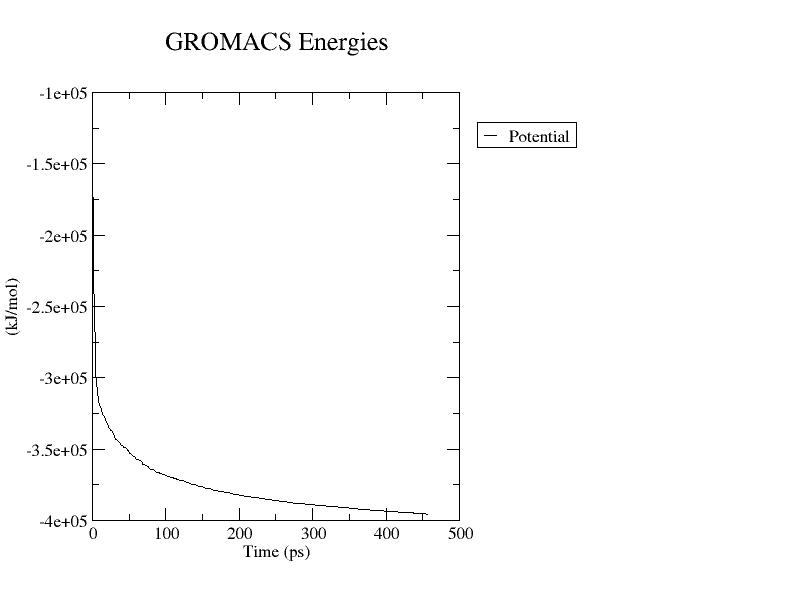
\includegraphics[width=\linewidth]{potential.jpg}
          \captionof{figure}{Energy Minimization I}
          \label{fig:Enrg1}
    \end{minipage}%
    \begin{minipage}{.5\textwidth}
          \centering
          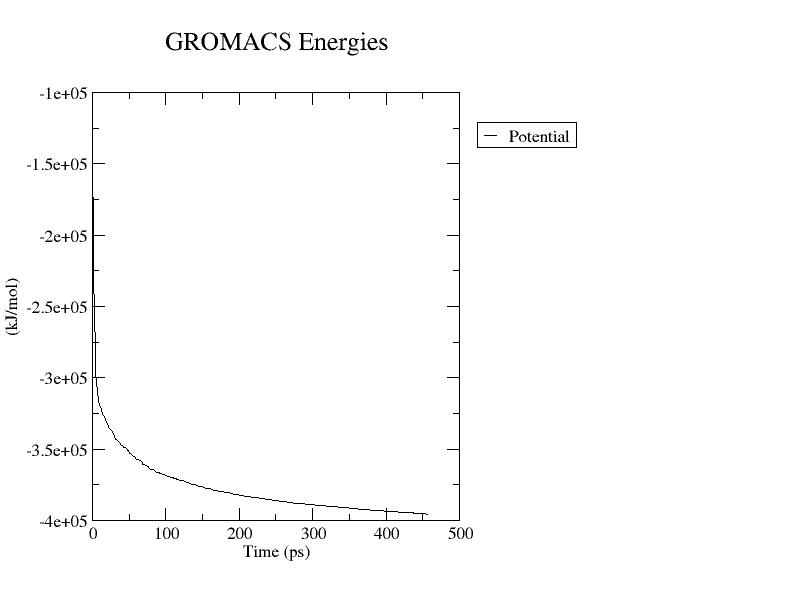
\includegraphics[width=\linewidth]{potential2.jpg}
          \captionof{figure}{Energy Minimization II}
          \label{fig:Enrg2}
    \end{minipage}
\end{figure}

 In order to start MD simulation we need to bring the system (solvent + solute) to equlibrium, we restrained the heavy atoms of the protein to move the solvent without the need to visit any conformation of the protein. Equilibrium is done in two phases with the first one conducted under NVT (constant number of particles, volume and temperature)\footnote{Also referred to as canonical or isothermal-isochoric} \cref{fig:temp}. The second phase is done under NPT (constant number of particles, pressure and temperature)\footnote{Aslo called isothermal-isobaric and is the closest to experimental conditions}. We then analyze the progression of pressure \cref{fig:prs}, and density \cref{fig:dens}
 
  \begin{figure}[H]
     \centering
     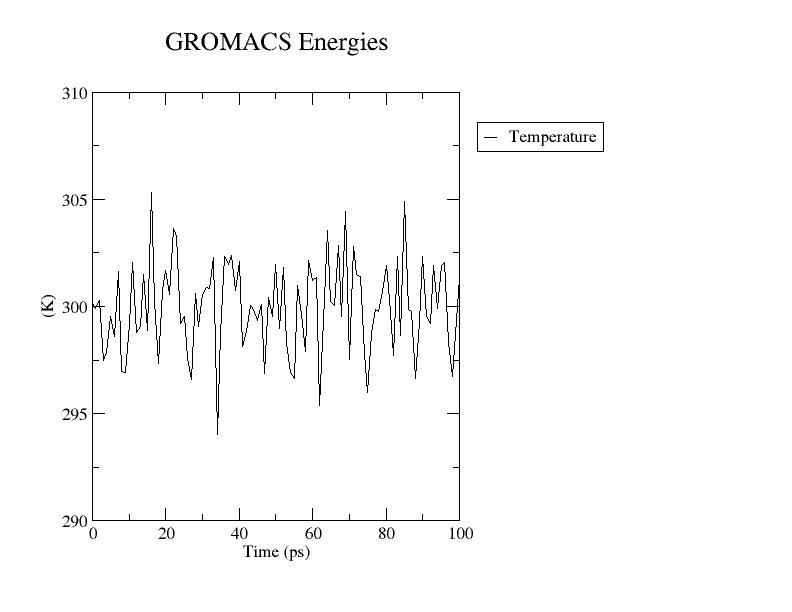
\includegraphics[width= \linewidth]{temperature.jpg}
     \caption{NVT Equilibration}
     \label{fig:temp}
 \end{figure}
 \begin{figure}[H]
    \begin{minipage}{.5\textwidth}
          \centering
          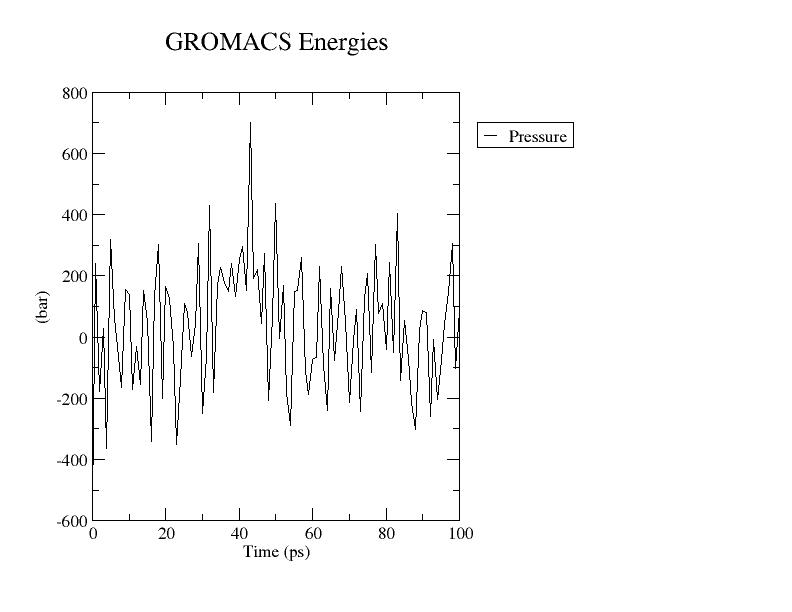
\includegraphics[width=\linewidth]{pressure.jpg}
          \captionof{figure}{NPT Equilibration : Pressure}
          \label{fig:prs}
    \end{minipage}%
    \begin{minipage}{.5\textwidth}
          \centering
          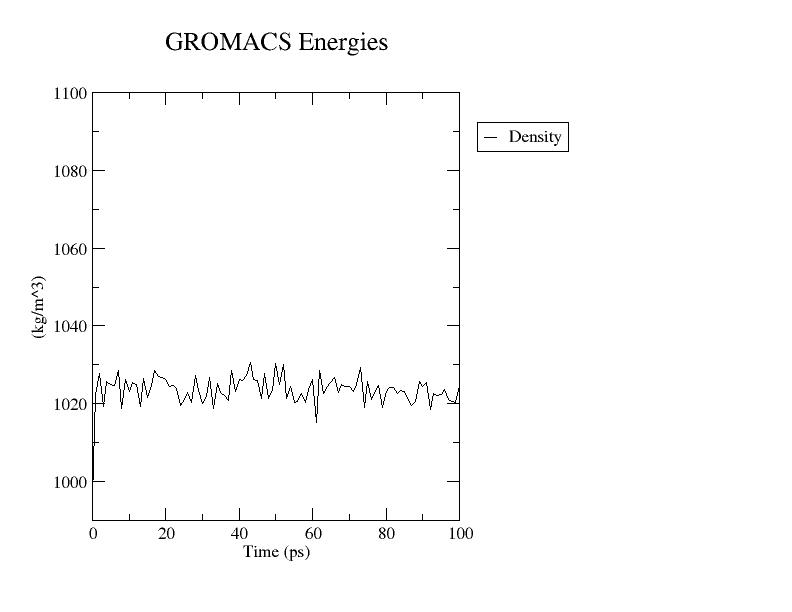
\includegraphics[width=\linewidth]{density.jpg}
          \captionof{figure}{NPT Equilibration : Density}
          \label{fig:dens}
    \end{minipage}
\end{figure}



%   \begin{figure}[H]
%      \centering
%      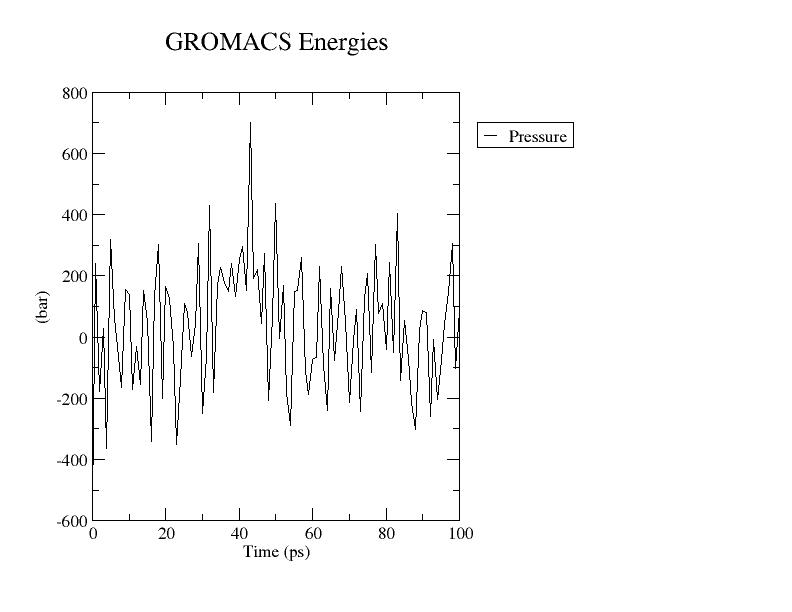
\includegraphics[width= \linewidth / 3]{pressure.jpg}
%      \caption{NPT Equilibration : Pressure}
%      \label{fig:prs}
%  \end{figure}
%  \begin{figure}[H]
%      \centering
%      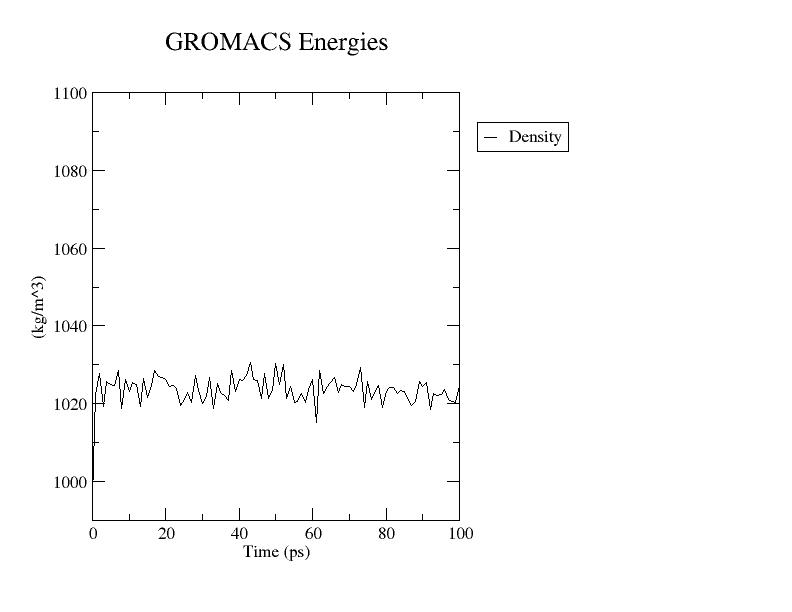
\includegraphics[width= \linewidth / 3]{density.jpg}
%      \caption{NPT Equilibration : Density}
%      \label{fig:dens}
%  \end{figure}
 Other text
 
 \section{Another Section}
 
\end{document}
